\documentclass{beamer}
\usetheme{Singapore}
% \setbeamersize{text margin left=5mm,text margin right=30mm} 
\usepackage{amsmath}
\usepackage[hyphens]{xurl}
\usepackage{changepage}

\title{Mathematical Modeling and Simulation of a Zombie Epidemic}
\subtitle{}
\author{Md Tariqul Islam}
\institute{Universit\"at Koblenz - Landau}
\date{November 10, 2021}

\setbeamertemplate{footline}
{
  \leavevmode%
  \hbox{%
  \begin{beamercolorbox}[wd=.2\paperwidth,ht=2.25ex,dp=1ex,center]{author in head/foot}%
    \usebeamerfont{author in head/foot}\insertshortauthor%~~\beamer@ifempty{\insertshortinstitute}{}{(\insertshortinstitute)}
  \end{beamercolorbox}%
  \begin{beamercolorbox}[wd=.49\paperwidth,ht=2.25ex,dp=1ex,center]{title in head/foot}%
    \usebeamerfont{title in head/foot}\insertshorttitle
  \end{beamercolorbox}%
  \begin{beamercolorbox}[wd=.3\paperwidth,ht=2.25ex,dp=1ex,right]{date in head/foot}%
    \usebeamerfont{date in head/foot}\insertshortdate{}\hspace*{2em}
    \insertframenumber{} / \inserttotalframenumber\hspace*{2ex} 
  \end{beamercolorbox}}%
  \vskip0pt%
}
    
\begin{document}

\begin{frame}
\titlepage
\end{frame}



\begin{frame}
\frametitle{Mathematical Modeling for Infectious Disease}
\begin{itemize}
	\item Describe disease scenario in terms of mathematical language
	
	\item Study the outbreak dynamics
	
	\item Predict the future flow
	
	\item Take informed decisions effectively and efficiently
\end{itemize}
\end{frame}



\begin{frame}
\frametitle{SIR Epidemic Model}

\begin{figure}[H]
\centering

\includegraphics[scale=1.0]{SIR.png}
\label{fig:SIR Model}
\end{figure}
~\\
\begin{equation*}
\begin{aligned}
&S^{\prime}(t)=-\beta SI \\
&I^{\prime}(t)=\beta SI - \alpha I \\
&R^{\prime}(t)=\alpha I \\
\end{aligned}
\end{equation*}

\tiny{Reference- [1]}
\end{frame}



\begin{frame}
\frametitle{SZR Model with Perturbation}

\begin{figure}[H]
\centering
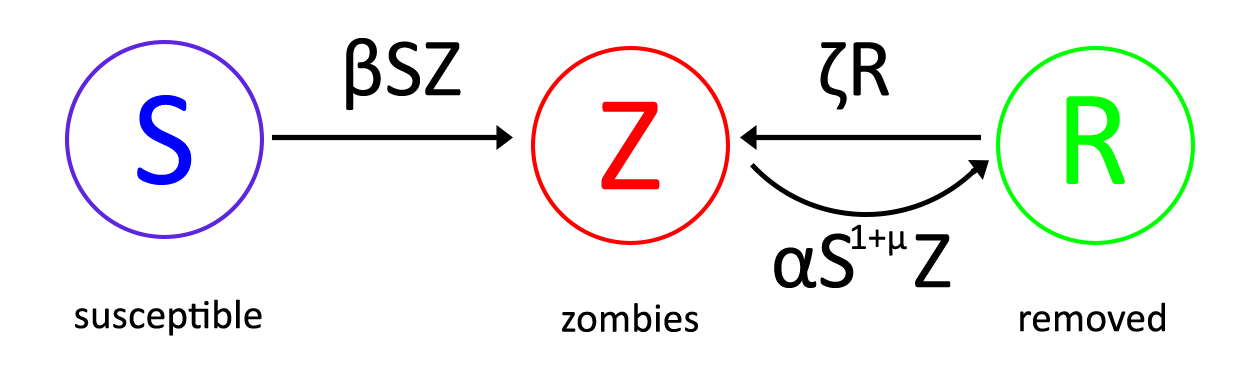
\includegraphics[scale=1.0]{SZR_mu.png}
\label{fig:Perturbed SZR Model}
\end{figure}
~\\
\begin{equation*}
\begin{aligned}
&S^{\prime}(t)=-\beta SZ \\
&Z^{\prime}(t)=\zeta R + \beta SZ - \alpha S^{1 + \mu} Z\\
&R^{\prime}(t)=\alpha S^{1 + \mu} Z - \zeta R \\
\end{aligned}
\end{equation*}

\tiny{Reference- [2], [3]}
\end{frame}



\begin{frame}
\begin{adjustwidth}{-1.5em}{-1.5em}
\frametitle{SZR Model- Graph Comparison}

\begin{figure}[H]
\centering
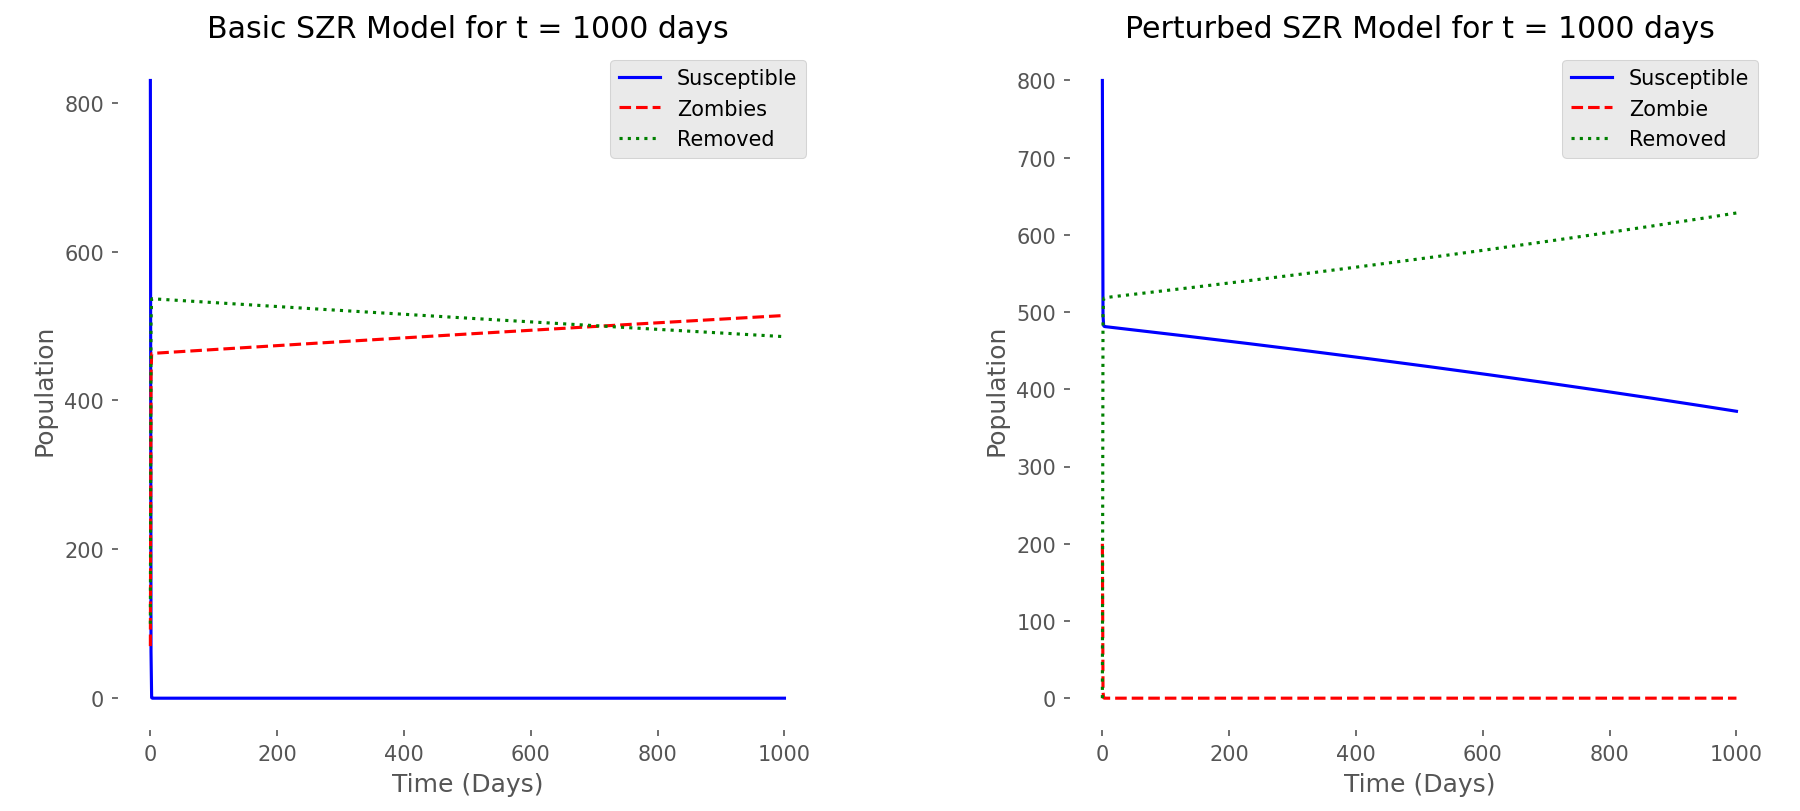
\includegraphics[scale=0.18]{SZRModel.png}
\label{fig:SZR Model 01}
\end{figure}
\end{adjustwidth}
\end{frame}



\begin{frame}
\begin{adjustwidth}{-1.5em}{-1.5em}
\frametitle{SZR Model with Perturbation- Perturbation Impacts}

\begin{figure}[H]
\centering
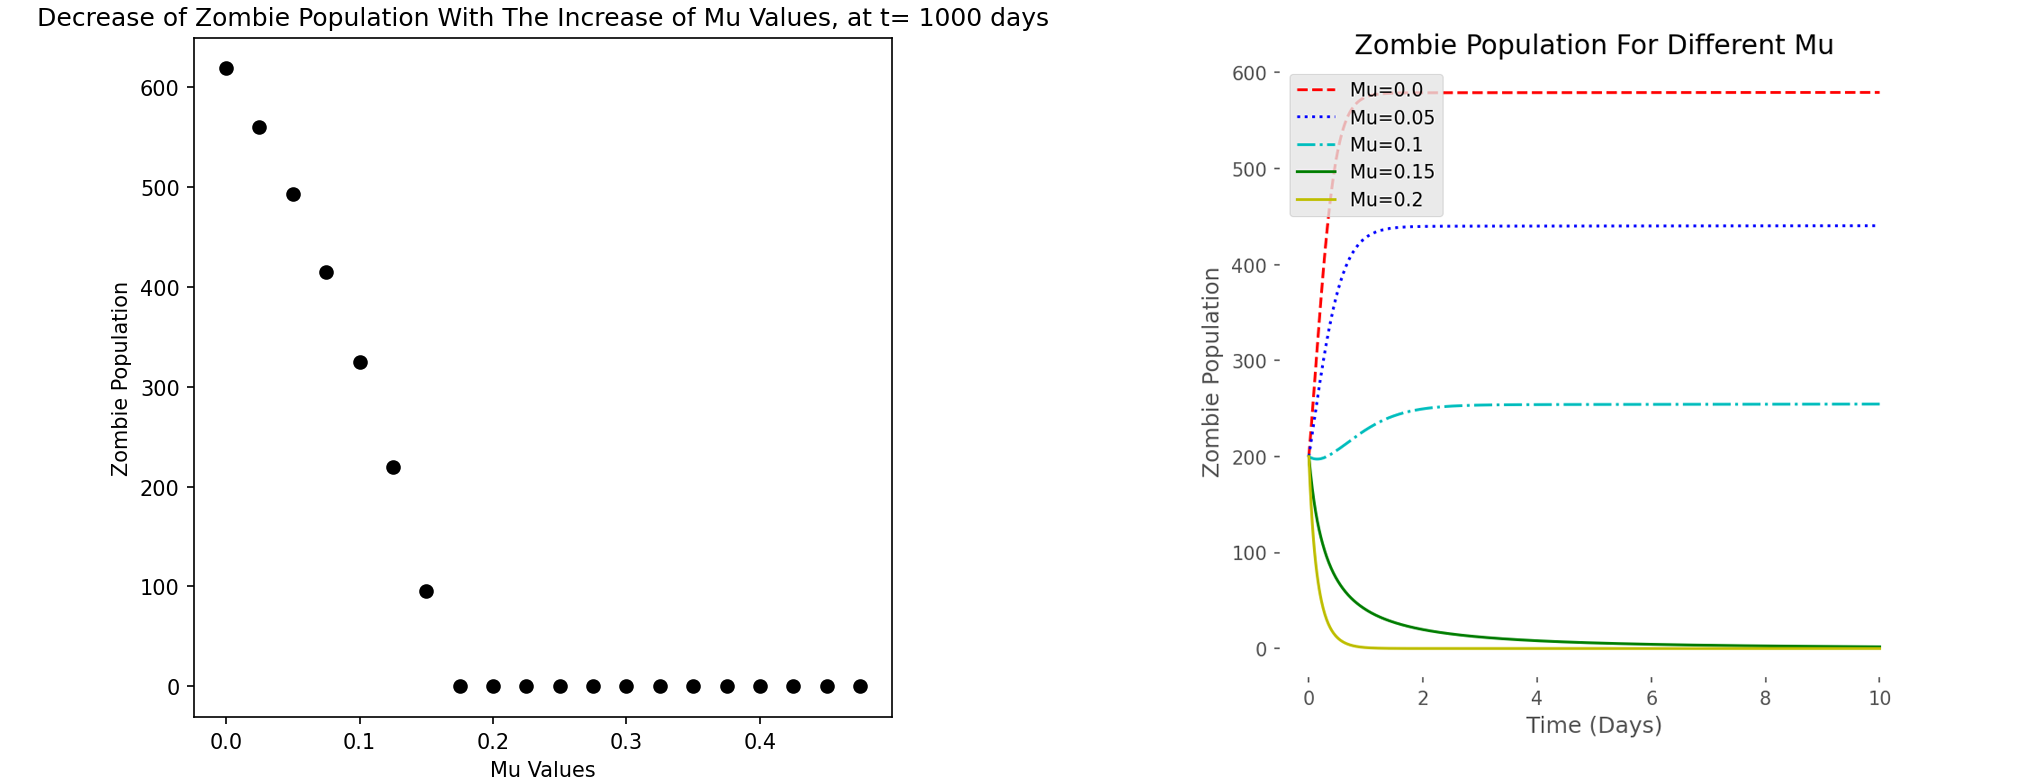
\includegraphics[scale=0.37]{SZR_3.png}
\label{fig:SZR Model 02}
\end{figure}
\end{adjustwidth}
\end{frame}



\begin{frame}
\frametitle{SZR Model with Perturbation- Graphical Interface Program}

\begin{figure}[H]
\centering
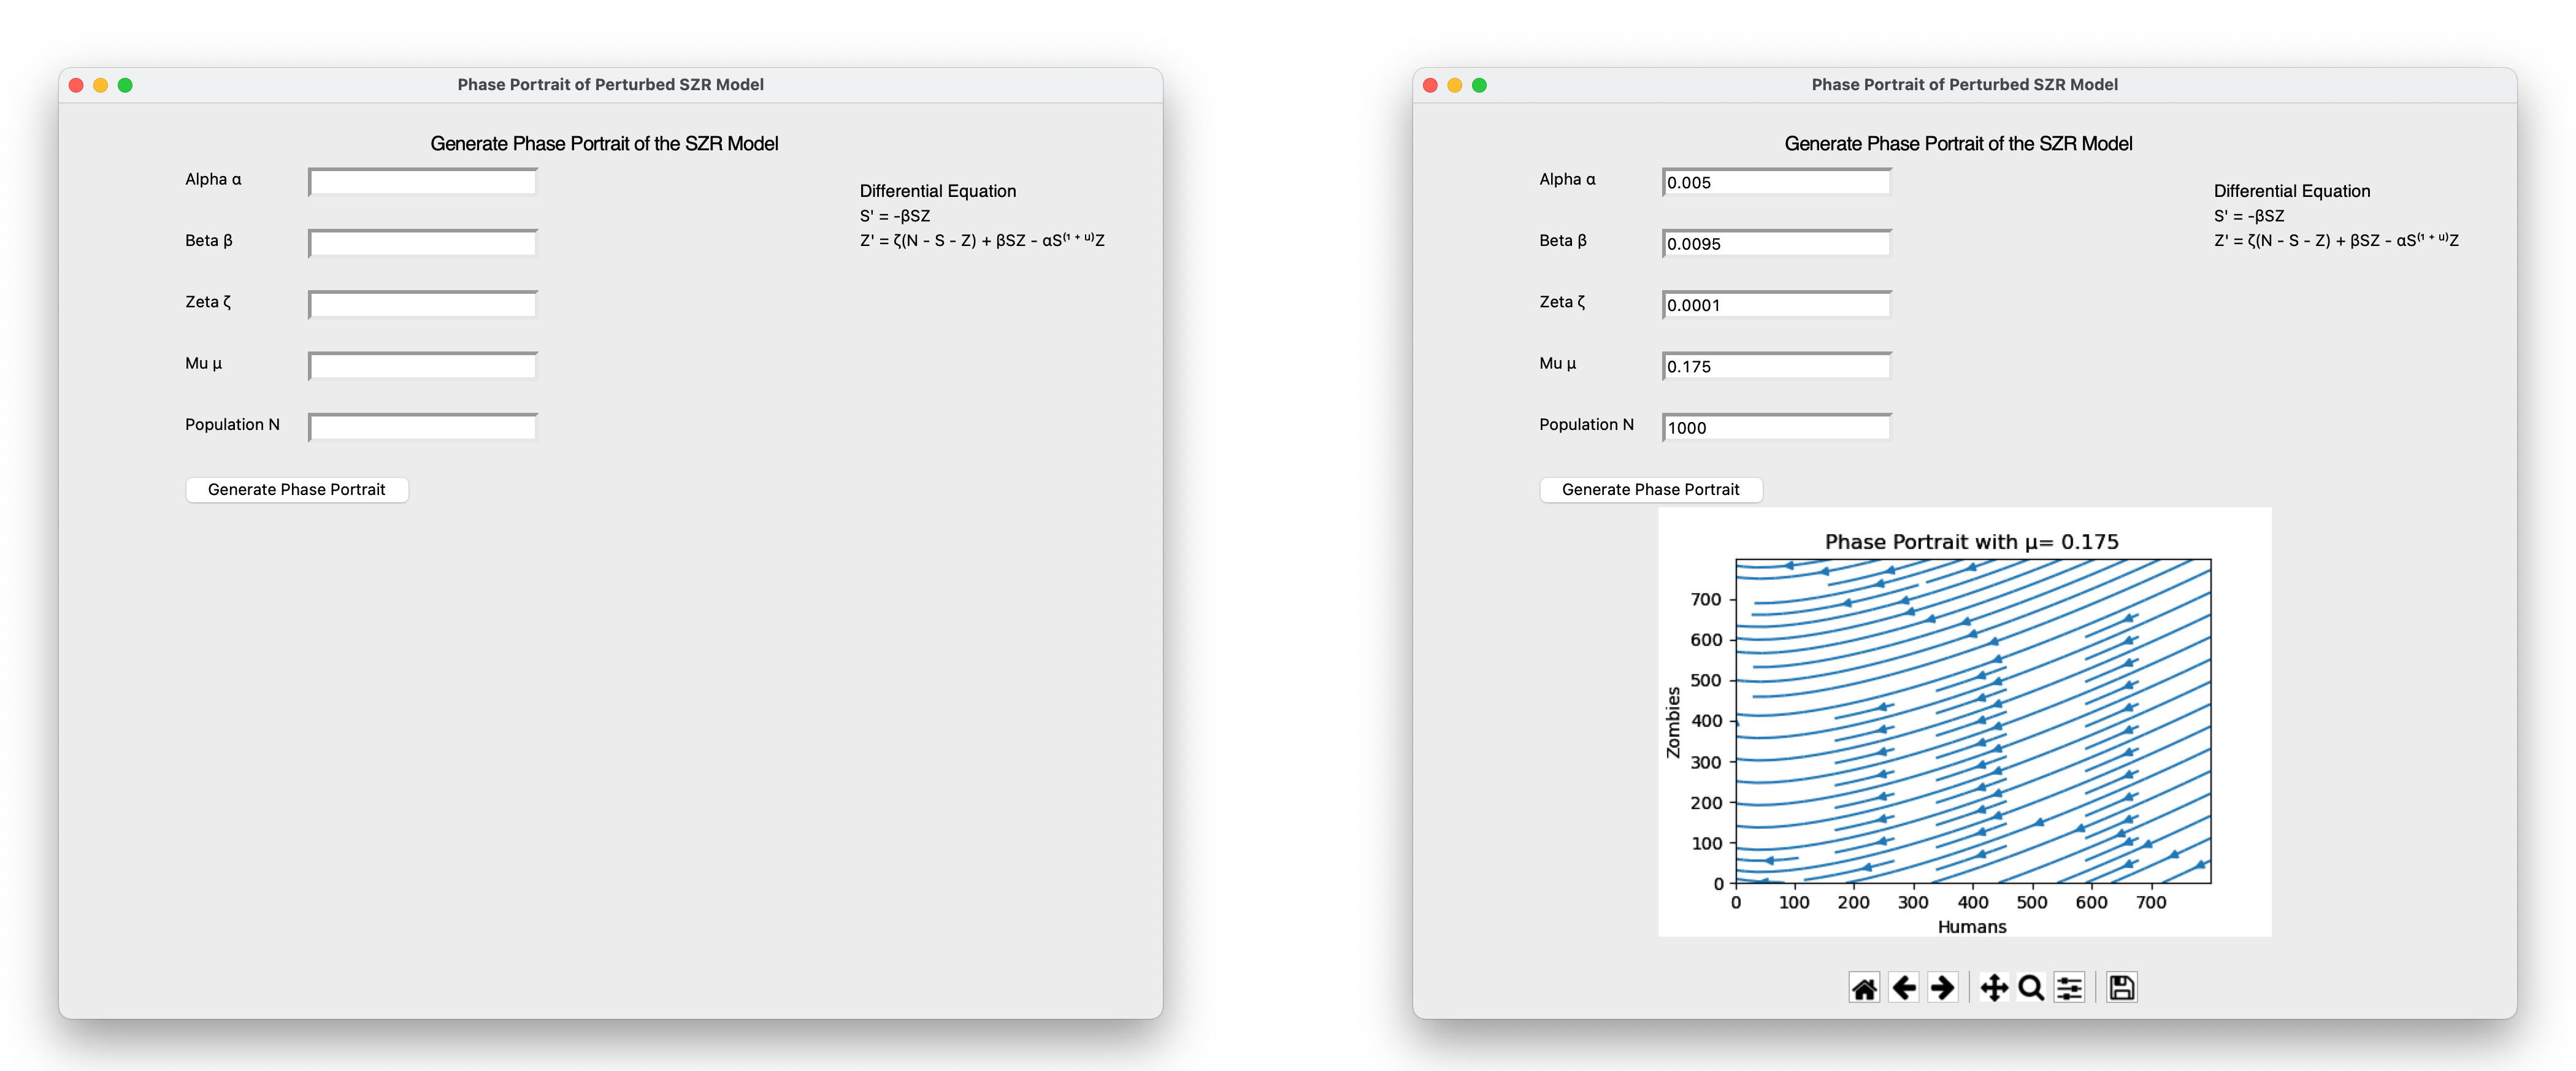
\includegraphics[scale=0.075]{SZR_2.png}
\label{fig:SZR Model 03}
\end{figure}
\end{frame}



\begin{frame}
\begin{adjustwidth}{-1.5em}{-1.5em}
\frametitle{Quarantine Model}


\begin{tabular}{cl}  
         \begin{tabular}{c}
           
\includegraphics[scale=0.5]{SEZQR.png}
           \end{tabular}
           & \begin{tabular}{l}
             \parbox{0.3\linewidth}{ 
             \begin{equation*}
\begin{split}
& S' = - \beta SZ \\
& E' = \beta SZ - (\rho + \kappa)E \\
& Z' = \rho E + \zeta R - \sigma Z - \alpha S^{1 + \mu} Z \\
& Q' = \kappa E + \sigma Z - \gamma Q \\
& R' = \alpha S^{1 + \mu} Z + \gamma Q - \zeta R \\
\end{split}
\end{equation*}
 }
         \end{tabular}  \\
\end{tabular}
\\

\tiny{Reference- [3]}
\end{adjustwidth}
\end{frame}



\begin{frame}
\begin{adjustwidth}{-2.0em}{-1.5em}
\frametitle{Modified Quarantine Model}

\begin{tabular}{cl}  
         \begin{tabular}{c}
           
\includegraphics[scale=0.42]{SEZQR_mu.png}
           \end{tabular}
           & \begin{tabular}{l}
             \parbox{0.4\linewidth}{ 
             \begin{equation*}
\begin{split}
& S' = - \beta SZ \\
& E' = \beta SZ - (\rho + \kappa)E \\
& Z' = \rho E + \zeta R - \sigma SZ - \alpha S^{1 + \mu} Z + \omega Q \\
& Q' = \kappa E + \sigma SZ - \gamma Q - \omega Q \\
& R' = \alpha S^{1 + \mu} Z + \gamma Q - \zeta R \\
\end{split}
\end{equation*}
 }
         \end{tabular}  \\
\end{tabular}
\end{adjustwidth}
\end{frame}



\begin{frame}
\frametitle{Modified Quarantine Model}

Basic Reproduction Number-- 
\begin{equation*}
\textit{R\textsubscript{0}}(\mu) = \frac{-\beta N[(\zeta-\rho)(\gamma+\omega)+\kappa(\zeta-\omega)]}{(\rho+\kappa)\left[(\gamma+\omega)\left(\alpha N^{1+\mu}+\sigma N+\zeta\right)+\sigma N(\zeta-\omega)\right]}
\end{equation*} \\
~\\
~\\
~\\
Condition for Disease Free Equilibrium--
\begin{equation*}
\mu>\frac{\ln \left(\frac{\beta N[(\zeta-\rho)(\gamma+\omega)+\kappa(\zeta-\omega)]+(\rho+\kappa)[\sigma N(\zeta-\omega)+(\gamma+\omega)(\zeta+\sigma N)]}{-\alpha(\gamma+\omega)(\rho+\kappa)}\right)}{\ln (N)}-1
\end{equation*}
\end{frame}



\begin{frame}
\begin{adjustwidth}{-1.7em}{-1.5em}
\frametitle{Modified Quarantine Model- Bifurcation Diagrams}

\begin{figure}[H]
\centering
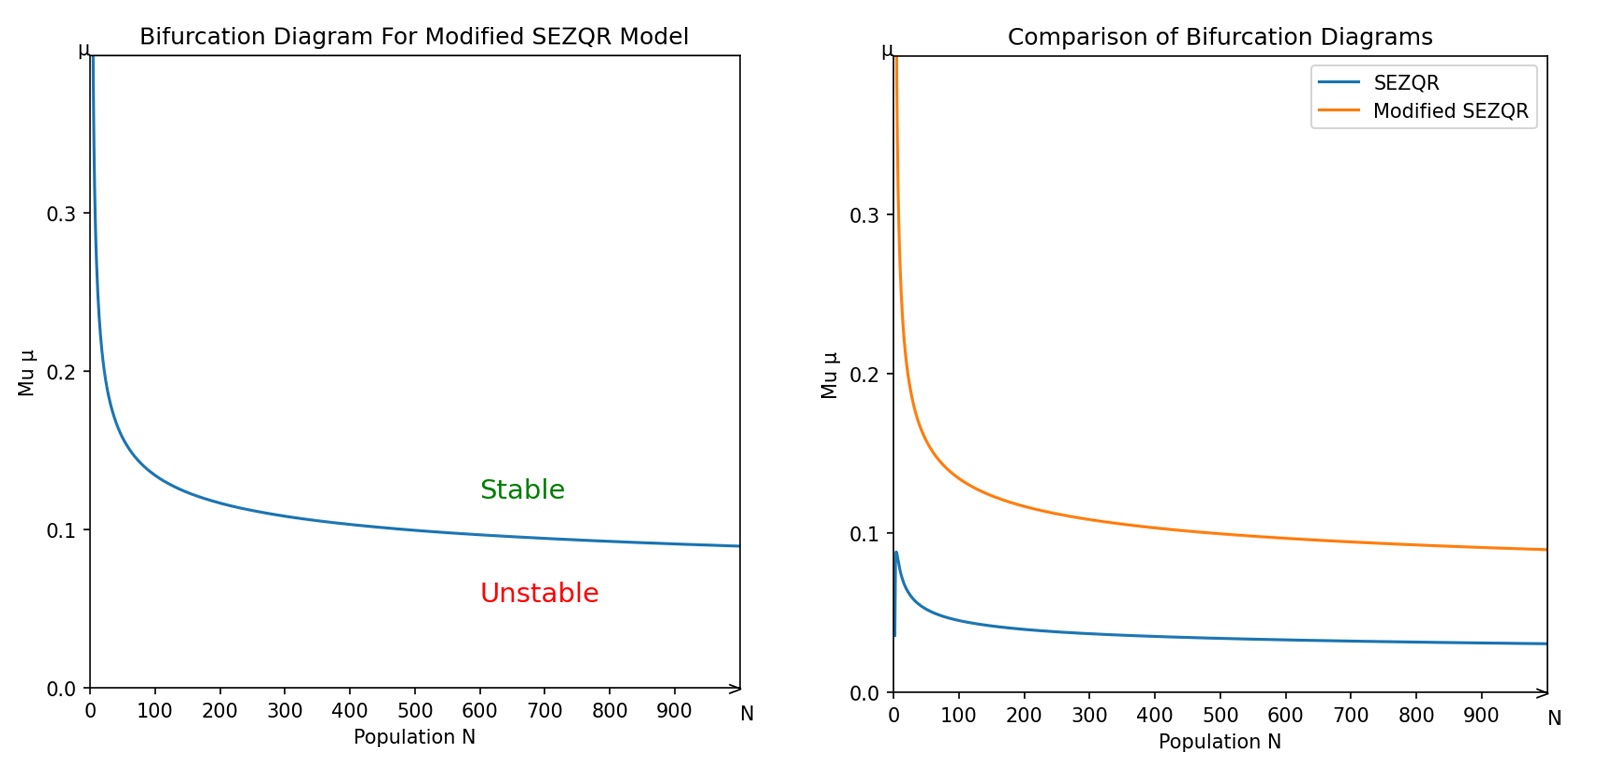
\includegraphics[scale=0.45]{SEZQR_3.png}
\label{fig:SEZQR Model 01}
\end{figure}
\end{adjustwidth}
\end{frame}



\begin{frame}
\begin{adjustwidth}{-1.7em}{-1.5em}
\frametitle{Modified Quarantine Model- Graph Comparison 01}

\begin{figure}[H]
\centering
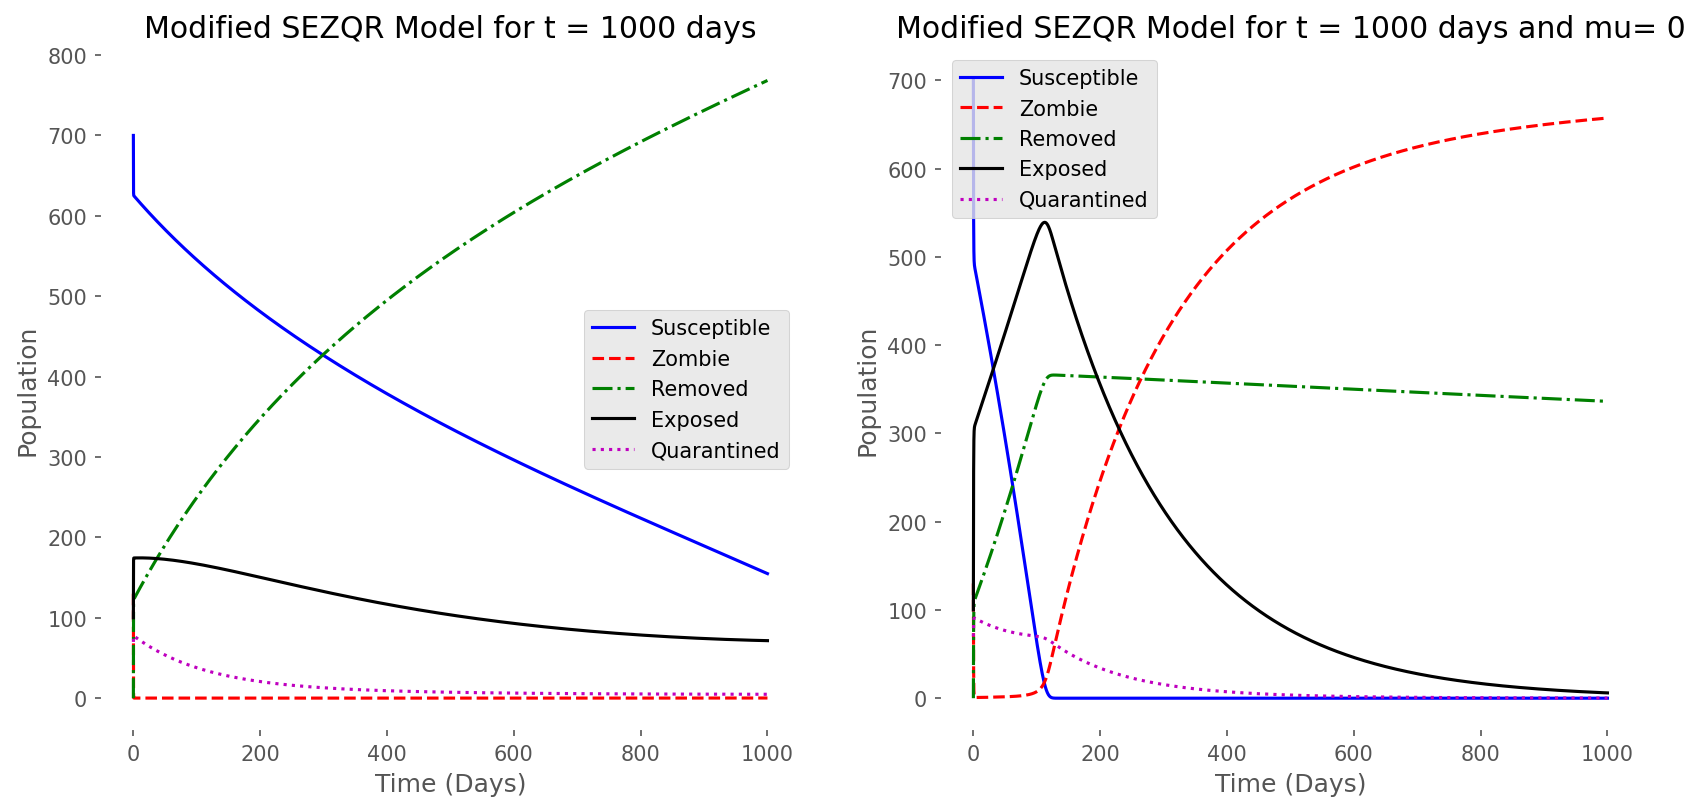
\includegraphics[scale=0.41]{SEZQR_1.png}
\label{fig:SEZQR Model 02}
\end{figure}
\end{adjustwidth}
\end{frame}



\begin{frame}
\begin{adjustwidth}{-1.7em}{-1.5em}
\frametitle{Modified Quarantine Model- Graph Comparison 02}

\begin{figure}[H]
\centering
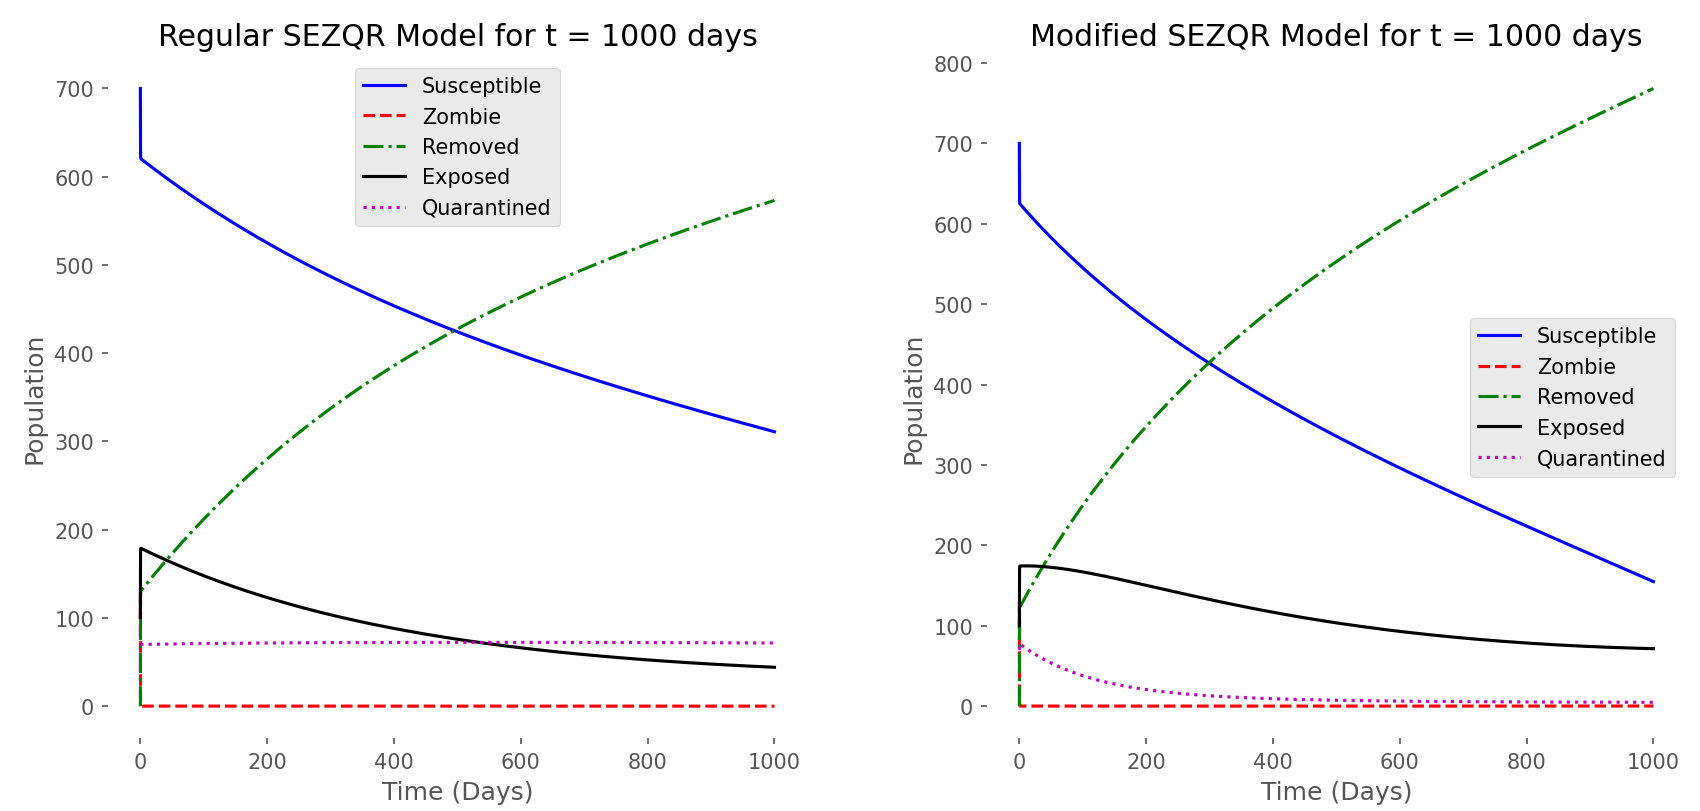
\includegraphics[scale=0.41]{Solution_Comparison.png}
\label{fig:SEZQR Model 03}
\end{figure}
\end{adjustwidth}
\end{frame}



\begin{frame}
\begin{adjustwidth}{-1.7em}{-1.5em}
\frametitle{Modified Quarantine Model- Perturbation Impacts}

\begin{figure}[H]
\centering
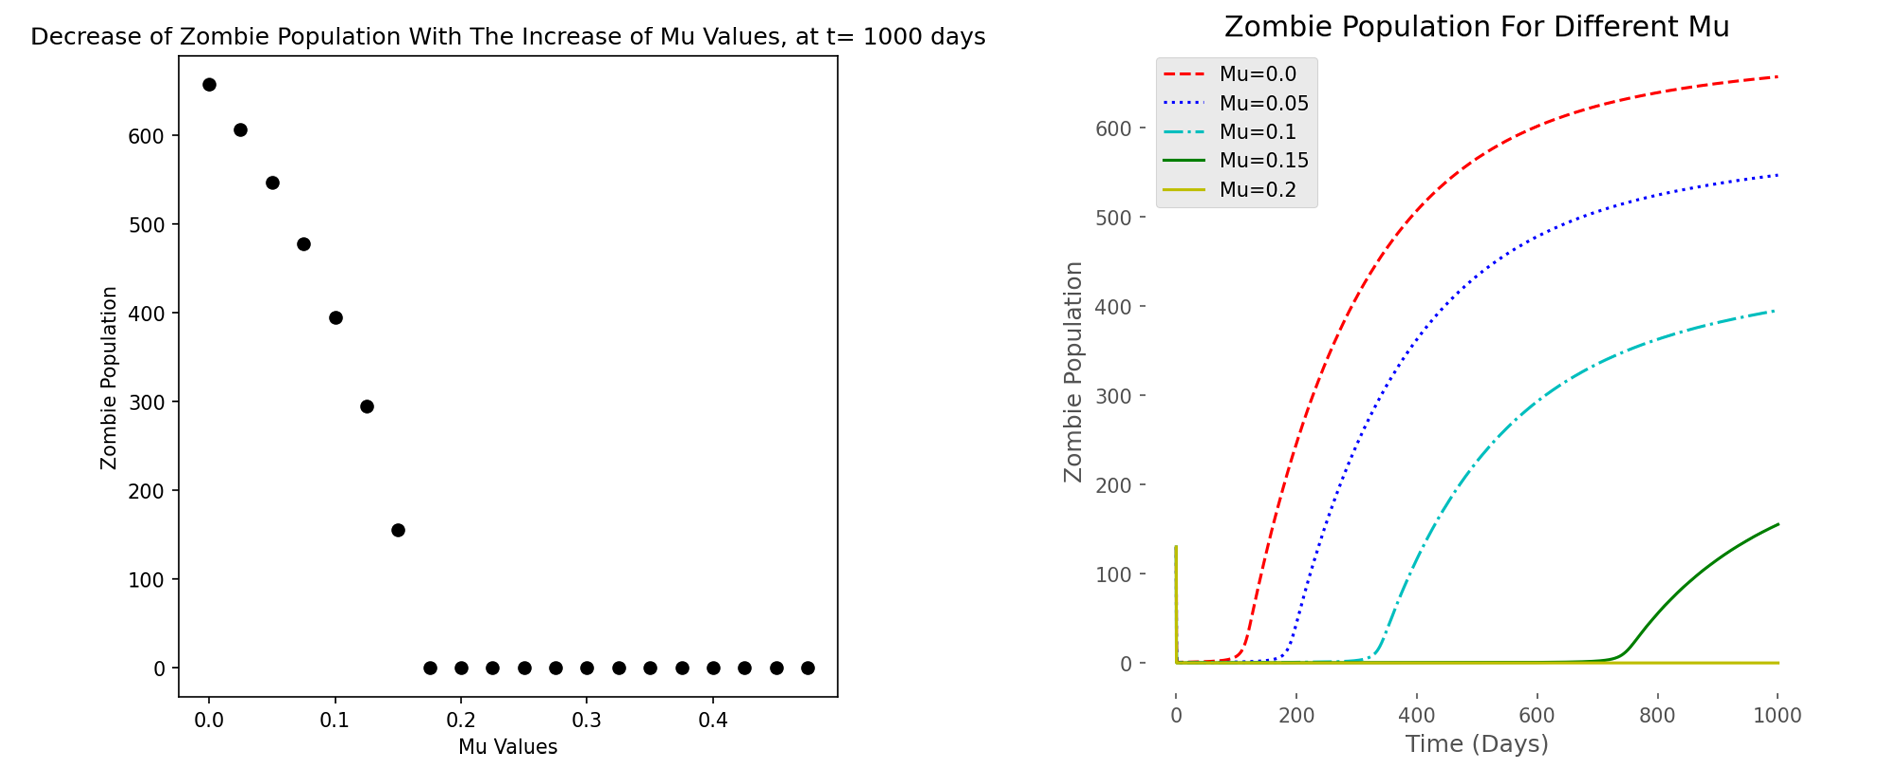
\includegraphics[scale=0.39]{SEZQR_2.png}
\label{fig:SEZQR Model 04}
\end{figure}
\end{adjustwidth}
\end{frame}



\begin{frame}
\frametitle{Conclusion}

\begin{itemize}
	\item Zombie epidemic can be a good approach to simulate real-world infectious disease outbreaks.
	
	\item Parameter estimates depend on real-world data.
	
	\item More variables and complications are needed to be considered to make the model more practical as well as pragmatic.
\end{itemize}
\end{frame}



\begin{frame}
\frametitle{References}

\scriptsize{[1] Kermack, W. O., \& McKendrick, A. G. (1927). A contribution to the mathematical theory of epidemics. Proceedings of the royal society of london. Series A, Containing papers of a mathematical and physical character, 115(772), 700-721. \\
URL- \url{https://doi.org/10.1098/rspa.1927.0118}} \\
~\\

\scriptsize{[2] Munz, P., Hudea, I., Imad, J., \& Smith, R. J. (2009). When zombies attack!: mathematical modelling of an outbreak of zombie infection. Infectious disease modelling research progress, 4, 133-150. \\
URL- \url{https://webspace.science.uu.nl/~frank011/Classes/modsim/Handouts/Zombies.pdf}}\\
~\\

\scriptsize{[3] Allen, R. F., Jens, C., \& Wendt, T. J. (2014). Perturbations in Epidemiological Models. Letters in Biomathematics, 1(2), 173-180. \\
URL- \url{https://doi.org/10.1080/23737867.2014.11414478}} \\
\end{frame}



\begin{frame}
\frametitle{}

\begin{center}
\textsc{\sffamily{\Large{Thank You}}}\\
\end{center}
\end{frame}



\begin{frame}
\frametitle{}

\begin{figure}[H]
\centering

\includegraphics[scale=0.6]{question.jpg}
\label{fig:question}
\end{figure}
\end{frame}



\begin{frame}
\begin{adjustwidth}{-1.7em}{-1.5em}
\frametitle{Backup Slide 01}

\begin{figure}[H]
\centering
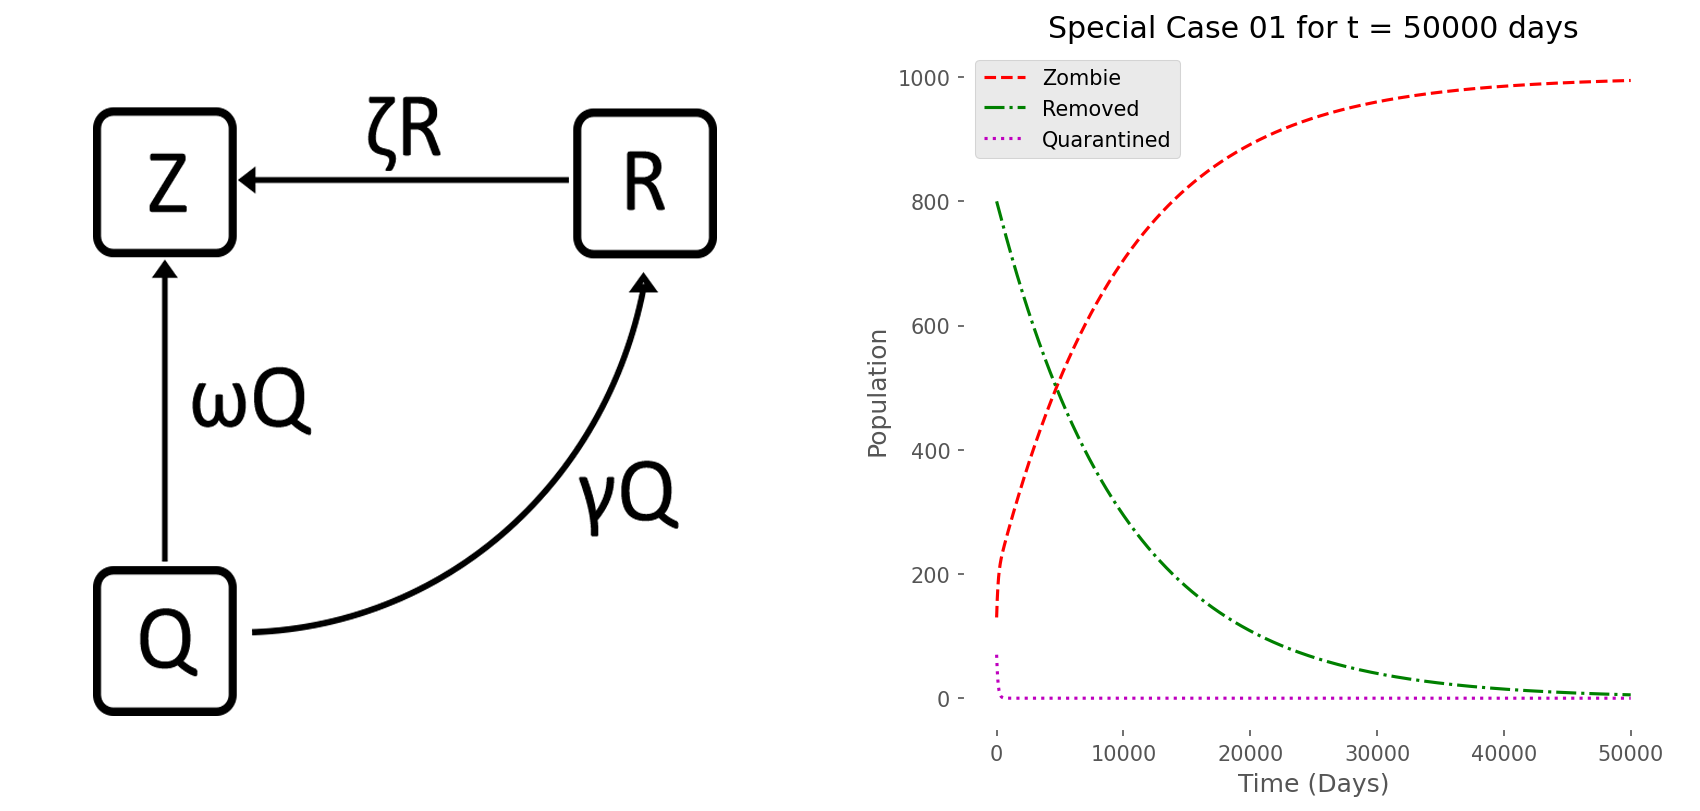
\includegraphics[scale=0.4]{special01.png}
\label{fig:backup01}
\end{figure}
\end{adjustwidth}
\end{frame}



\begin{frame}
\frametitle{Backup Slide 02}

\begin{figure}[H]
\centering
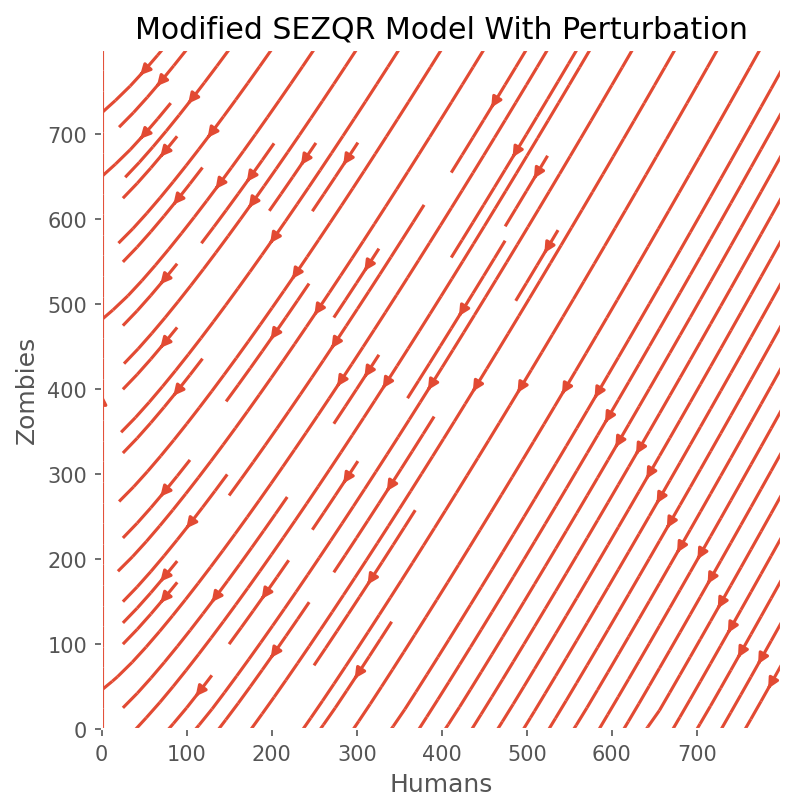
\includegraphics[scale=0.5]{ModifiedSEZQR_PhasePortrait.png}
\label{fig:backup02}
\end{figure}
\end{frame}



\begin{frame}
\begin{adjustwidth}{-1.7em}{-1.5em}
\frametitle{Backup Slide 03}

\begin{figure}[H]
\centering
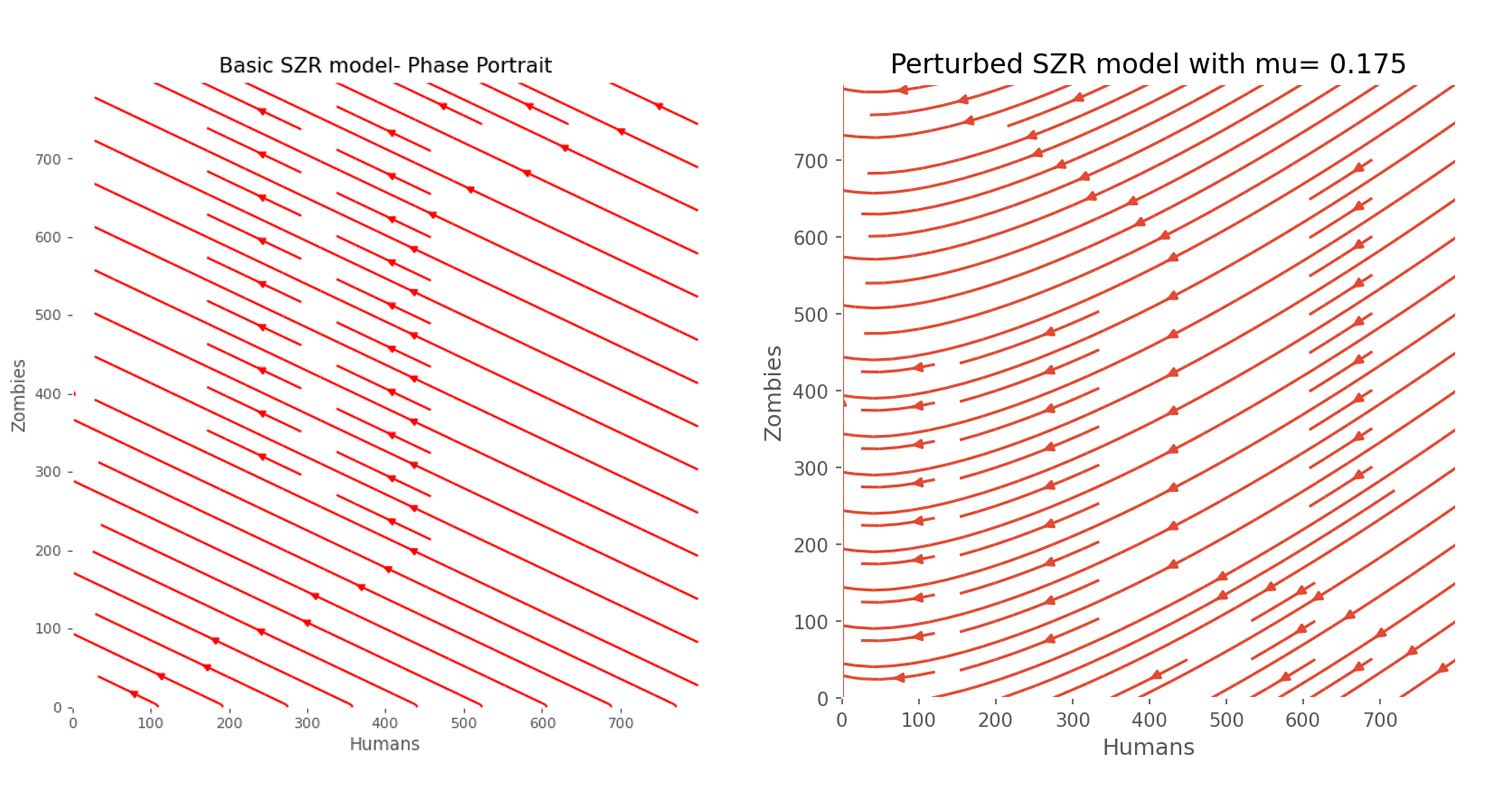
\includegraphics[scale=0.45]{special02.png}
\label{fig:backup03}
\end{figure}
\end{adjustwidth}
\end{frame}



\begin{frame}
\begin{adjustwidth}{-1.7em}{-1.5em}
\frametitle{Backup Slide 04}

\begin{figure}[H]
\centering
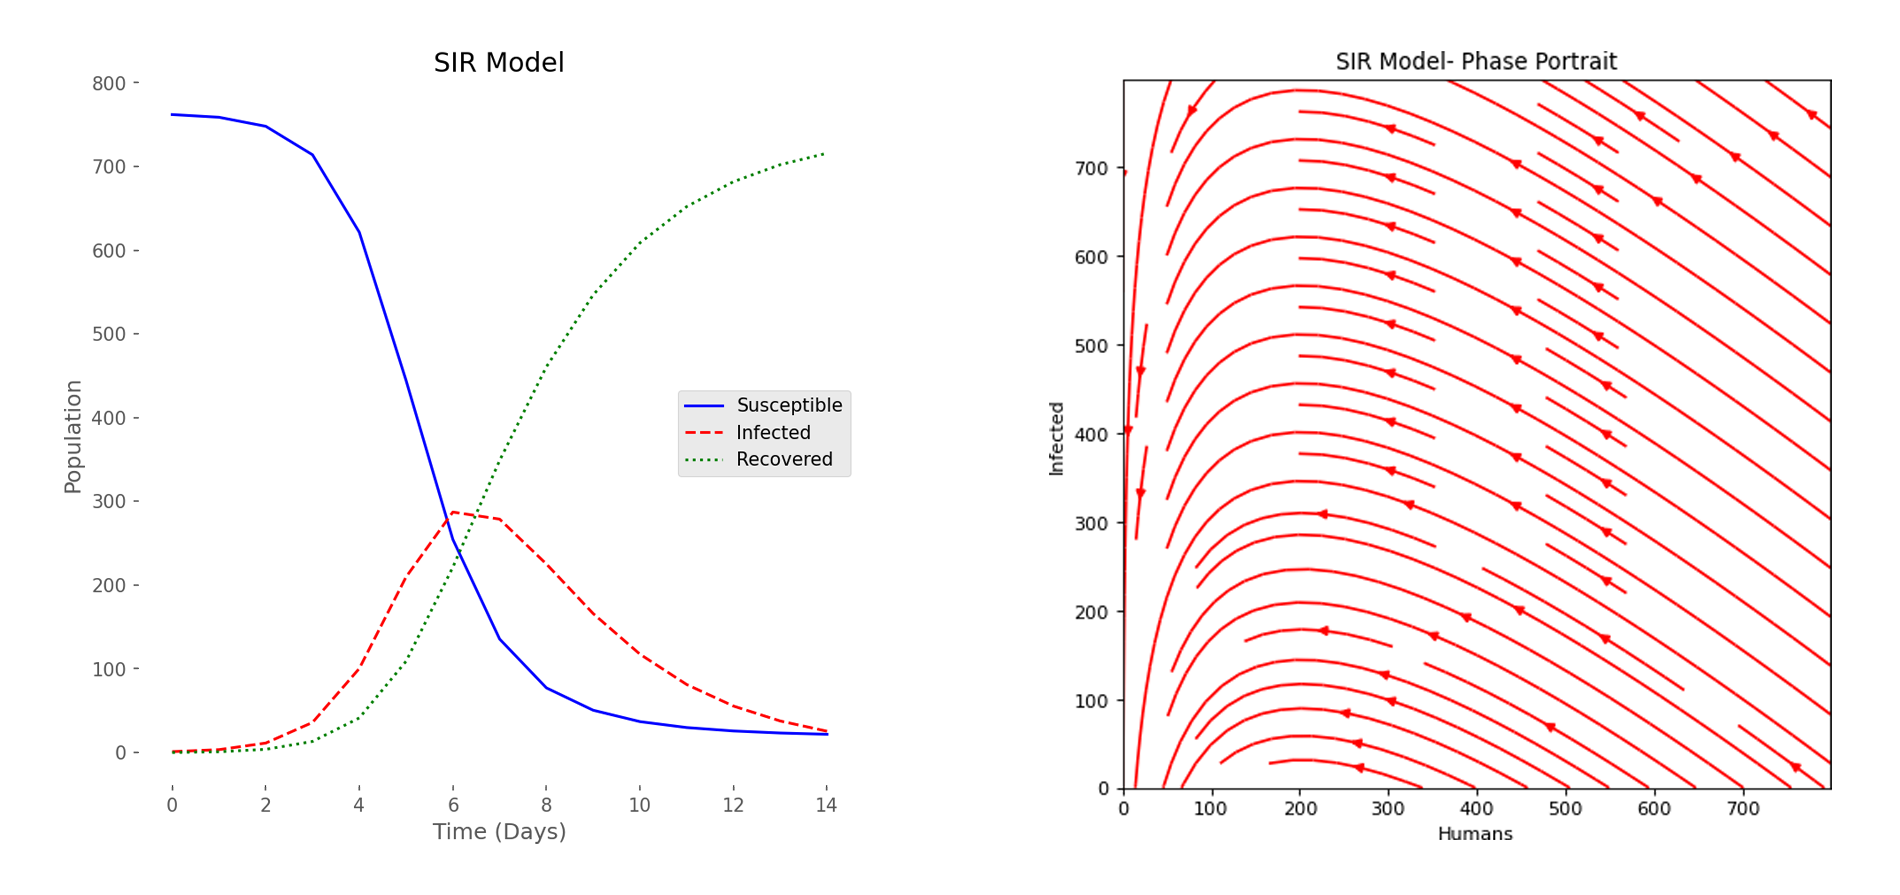
\includegraphics[scale=0.38]{special03.png}
\label{fig:backup04}
\end{figure}
\end{adjustwidth}
\end{frame}

\end{document}

